\textit{Cette dernière partie présente Symfony2, le framework utilisé pour le développement de cette application. Elle détaille également la structure et les entités créées, ainsi que le schéma relationnel généré par l'ORM Doctrine2, intégré dans le framework. Enfin, les vue finales sont présentées.}

\section{Le framework Symfony2}
\subsection{Présentation du framework}
Symfony est un framework PHP développé par l'équipe française SensioLabs dirigée par Fabien Potencier. Le but d'un tel outil est d’accélérer le développement et l'accélération d'applications web en se basant sur MVC\footnote{Modèle Vue Contrôleur}, patron de conception classiquement utilisé dans les applications modernes.

Il s'agit d'un outil open source qui rassemble divers projets reconnus (Mojavi pour le coté MVC, Doctrine pour la partie ORM, Twig pour le moteur de template).

Le projet, créé en 1998, a atteint aujourd'hui une grande maturité. Pour preuve l'utilisation de ce framework par Yahoo et Dailymotion.

Pour ce projet, nous avons utilisé la deuxième version de Symfony (Symfony2).

\subsection{Structure}

\subsubsection{Bundle}
Il s'agit d'un module ou d'un plugin :
\begin{itemize}
\item portable,
\item facilement installable dans un projet Symfony2,
\item qui possède une architecture MVC.
\end{itemize}

Un bundle ne possède pas de définition exacte. Il peut être vu comme un projet à part entière, une partie d'un projet, un plugin, etc\ldots

Chaque Bundle possède des vues, des entitées, des contrôleurs, etc\ldots

\subsubsection{Entity}
Une entité (Entity) est une classe présente dans un Bundle. Elle peut être en relation avec l'ORM afin d'être persistante, posséder des formulaires, être associée à des actions ou à des vues.

\subsection{L'ORM Doctrine2}

Doctrine2 est un des ORM le plus utilisé à ce jour. Il est sous licence libre GNU LGPL. C'est l'ORM par défaut de Symfony depuis la version 1.3. Parfaitement intégré au framework, les entités créées dans les Bundles Symfony peuvent contenir des tags qui permettent de dialoguer avec Doctrine et de définir la clé primaire, les relations, les types de champs, etc\ldots

\section{Structure de \emph{Thésaurus Rex}}

Pour le développement de cette application, nous avons créé un Bundle nommé \emph{ProjetBDDThesaurusBundle}, contenant lui même les deux entités déclarées dans notre diagramme de classe final : \emph{Terme} et \emph{Concept}.

\subsection{Entité \emph{Terme}}
\lstinputlisting[language=PHP,morekeywords={class, public, function, return, private, namespace, use}]{../../App/Symfony/src/ProjetBDD/Thesaurus/Bundle/Entity/Terme.php}

\subsection{Entité \emph{Concept}}
\lstinputlisting[language=PHP,morekeywords={class, public, function, return, private, namespace, use}]{../../App/Symfony/src/ProjetBDD/Thesaurus/Bundle/Entity/Concept.php}

\section{Schéma relationnel généré}

\subsection{Schéma simplifié}
\begin{description}
\item[terme](\underline{id})
\item[concept](\underline{id}, terme\_vedette\_id\up{\#}, concept\_general\_id\up{\#}) (Impossibilité de mettre en clé primaire une clé étrangère :s)
\item[concept\_terme](\underline{concept\_id\up{\#}, terme\_id\up{\#}})
\item[concept\_concept](\underline{concept1\_id\up{\#}, concept2\_id\up{\#}})
\end{description}

\subsection{Schéma complet}
\begin{verbatim}
thibaut=> \d+ terme
                          Table « public.terme »
 Colonne |          Type          | Modificateurs | Stockage 
---------+------------------------+---------------+----------
 id      | character varying(255) | non NULL      | extended  
Index :
    "terme_pkey" PRIMARY KEY, btree (id)
Référencé par :
    TABLE "concept" CONSTRAINT "fk_28f759cce6a95e6d" FOREIGN KEY (t
erme_vedette_id) REFERENCES terme(id)
    TABLE "concept_terme" CONSTRAINT "fk_3bf6677a26062764" FOREIGN 
KEY (terme_id) REFERENCES terme(id) ON DELETE CASCADE
Contient des OID: non

thibaut=> \d+ concept
                                          Table « public.concept »
      Colonne       |          Type          |  Modificateurs   | Stockage  
--------------------+------------------------+------------------+----------
 id                 | integer                | non NULL         | plain    
 terme_vedette_id   | character varying(255) | Par défaut, NULL | extended
 concept_general_id | integer                |                  | plain     
Index :
    "concept_pkey" PRIMARY KEY, btree (id)
    "idx_28f759ccd859483c" btree (concept_general_id)
    "idx_28f759cce6a95e6d" btree (terme_vedette_id)
Contraintes de clés étrangères :
    "fk_28f759ccd859483c" FOREIGN KEY (concept_general_id) REFERENC
ES concept(id)
    "fk_28f759cce6a95e6d" FOREIGN KEY (terme_vedette_id) REFERENCES
 terme(id)
Référencé par :
    TABLE "concept" CONSTRAINT "fk_28f759ccd859483c" FOREIGN KEY (c
oncept_general_id) REFERENCES concept(id)
    TABLE "concept_terme" CONSTRAINT "fk_3bf6677af909284e" FOREIGN 
KEY (concept_id) REFERENCES concept(id) ON DELETE CASCADE
    TABLE "concept_concept" CONSTRAINT "fk_79a50ccb47f1482c" FOREIG
N KEY (concept1_id) REFERENCES concept(id)
    TABLE "concept_concept" CONSTRAINT "fk_79a50ccb5544e7c2" FOREIG
N KEY (concept2_id) REFERENCES concept(id)
Triggers :
    tgr_verif_root AFTER DELETE OR UPDATE ON concept FOR EACH ROW E
XECUTE PROCEDURE fc_verif_root()
Contient des OID: non

thibaut=> \d+ concept_terme
                        Table « public.concept_terme »
  Colonne   |          Type          | Modificateurs | Stockage 
------------+------------------------+---------------+----------
 concept_id | integer                | non NULL      | plain     
 terme_id   | character varying(255) | non NULL      | extended  
Index :
    "concept_terme_pkey" PRIMARY KEY, btree (concept_id, terme_id)
    "idx_3bf6677a26062764" btree (terme_id)
    "idx_3bf6677af909284e" btree (concept_id)
Contraintes de clés étrangères :
    "fk_3bf6677a26062764" FOREIGN KEY (terme_id) REFERENCES terme(i
d) ON DELETE CASCADE
    "fk_3bf6677af909284e" FOREIGN KEY (concept_id) REFERENCES conce
pt(id) ON DELETE CASCADE
Contient des OID: non

thibaut=> \d+ concept_concept
                Table « public.concept_concept »
   Colonne   |  Type   | Modificateurs | Stockage 
-------------+---------+---------------+----------
 concept1_id | integer | non NULL      | plain     
 concept2_id | integer | non NULL      | plain     
Index :
    "concept_concept_pkey" PRIMARY KEY, btree (concept1_id, concept2_id)
    "idx_79a50ccb47f1482c" btree (concept1_id)
    "idx_79a50ccb5544e7c2" btree (concept2_id)
Contraintes de clés étrangères :
    "fk_79a50ccb47f1482c" FOREIGN KEY (concept1_id) REFERENCES concept(id)
    "fk_79a50ccb5544e7c2" FOREIGN KEY (concept2_id) REFERENCES concept(id)
Triggers :
    tgr_gestion_relations AFTER INSERT OR DELETE OR UPDATE ON concept_concept FOR EACH ROW EXECUTE PROCEDURE fc_gestion_relations()
Contient des OID: non

\end{verbatim}

\subsection{Ajout d'un déclencheur}

Dans le but de gérer la symétrie des associations entre concepts (table \texttt{concept\_concept}), nous avons développé un déclencheur qui :
\begin{itemize}
\item lors d'un \texttt{INSERT} ajoute l'association symétrique,
\item lors d'un \texttt{UPDATE} modifie l'association symétrique correspondante,
\item lors d'un \texttt{DELETE} supprime l'association symétrique correspondante.
\end{itemize}

Ce déclencheur assure l'intégrité des relations à tout moment.

\subsubsection{Script de mise en place du déclencheur}
\lstinputlisting[language=sql,morekeywords={REPLACE,FUNCTION,RETURNS,IF,ELSEIF,RETURN,LANGUAGE,DECLARE,BEGIN,FOR,EACH,ROW,PROCEDURE}]{./sources/trigger.sql}

\section{Templates finaux}

Les templates sont réalisés en HTML5 / CSS3. Nous avons tenu à rester fidèle aux vue réalisées lors de la conception.

\subsubsection{Accueil}
\begin{figure}[H]
\begin{center}
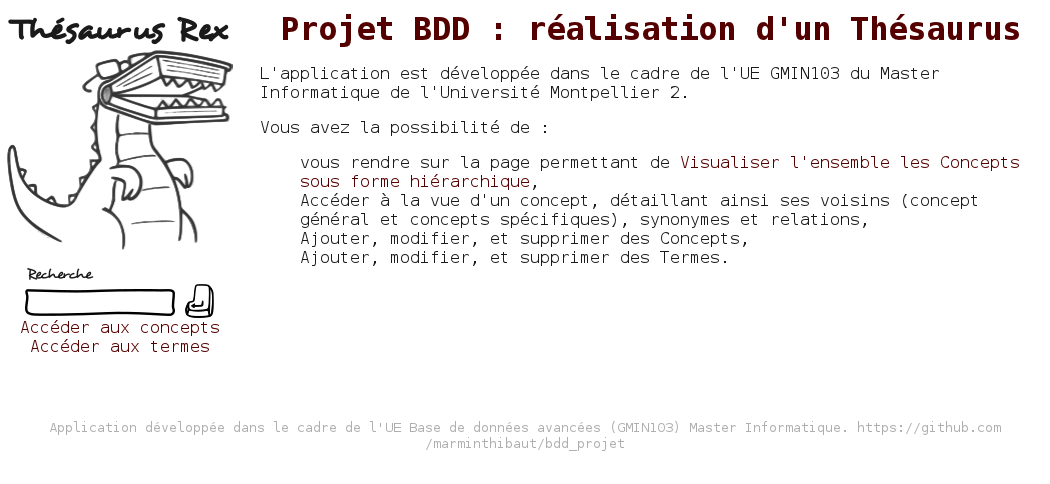
\includegraphics[width=\textwidth]{files/screen_accueil}
\end{center}
\caption{Aperçu de la page d'accueil.}
\end{figure}

\subsubsection{Liste des concepts}
\begin{figure}[H]
\begin{center}
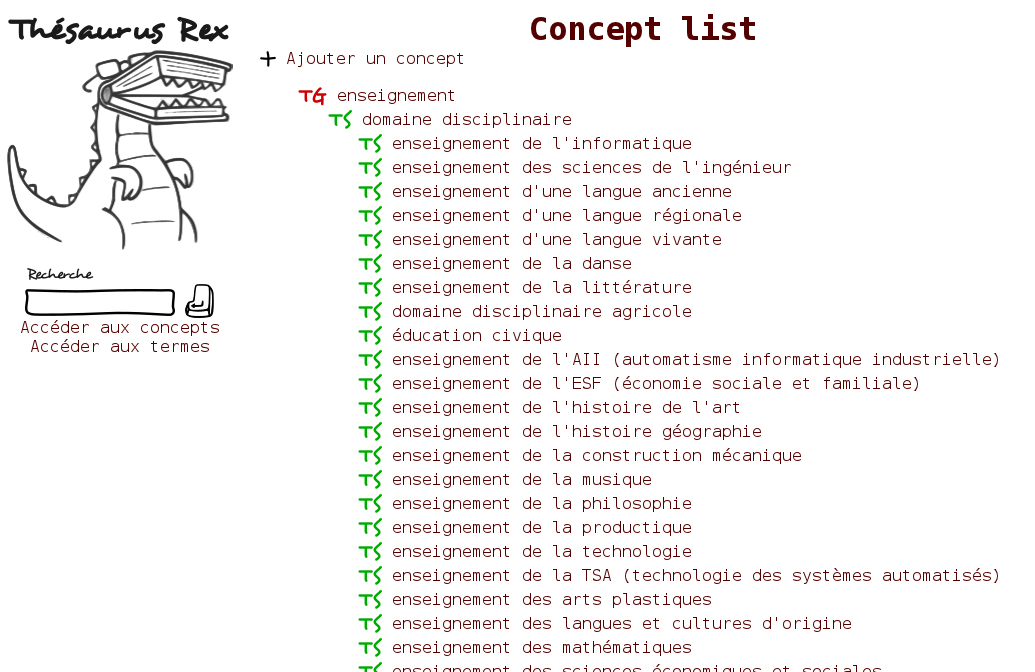
\includegraphics[width=\textwidth]{files/screen_concepts}
\end{center}
\caption{Hiérarchie des concepts.}
\end{figure}

\subsubsection{Affichage d'un concept}
\begin{figure}[H]
\begin{center}
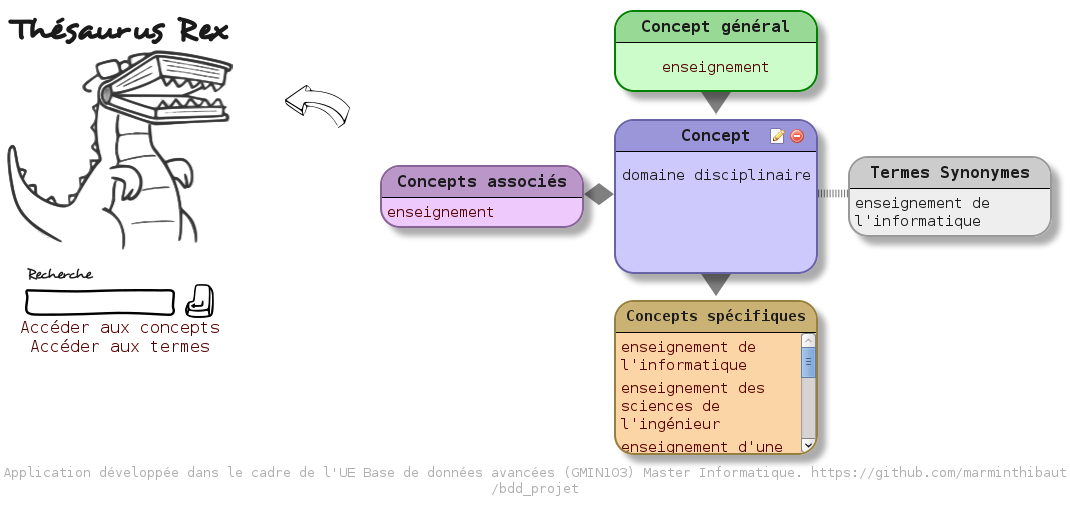
\includegraphics[width=\textwidth]{files/screen_concept}
\end{center}
\caption{Aperçu de la page d'un concept.}
\end{figure}

\subsubsection{Modification d'un concept}
\begin{figure}[H]
\begin{center}
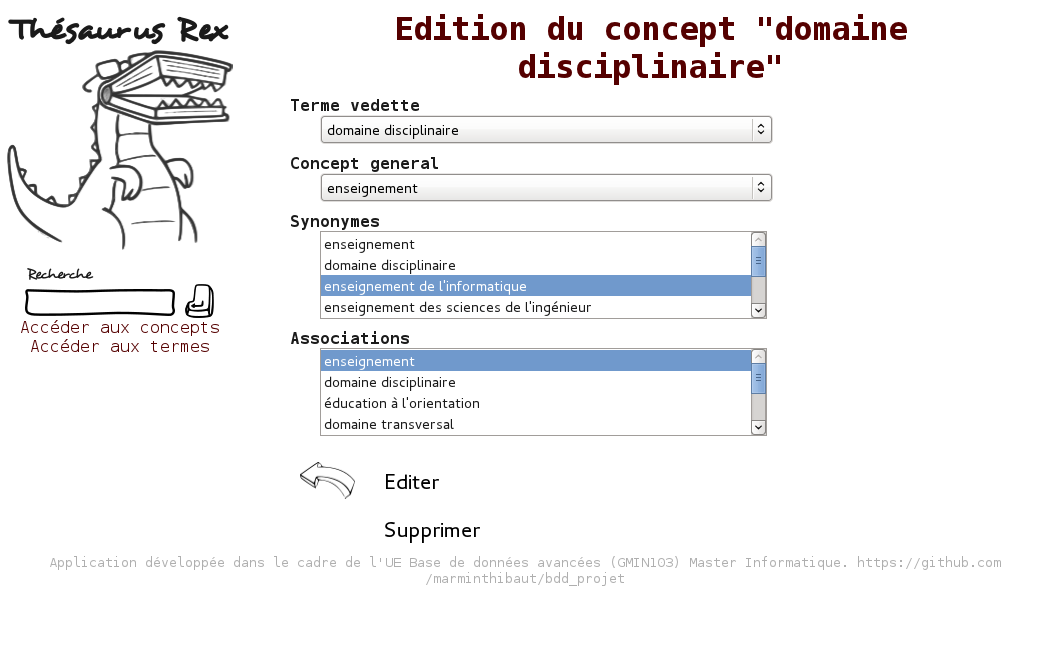
\includegraphics[width=\textwidth]{files/screen_concept_edit}
\end{center}
\caption{Formulaire de modification d'un concept.}
\end{figure}

\subsubsection{Liste des termes}
\begin{figure}[H]
\begin{center}
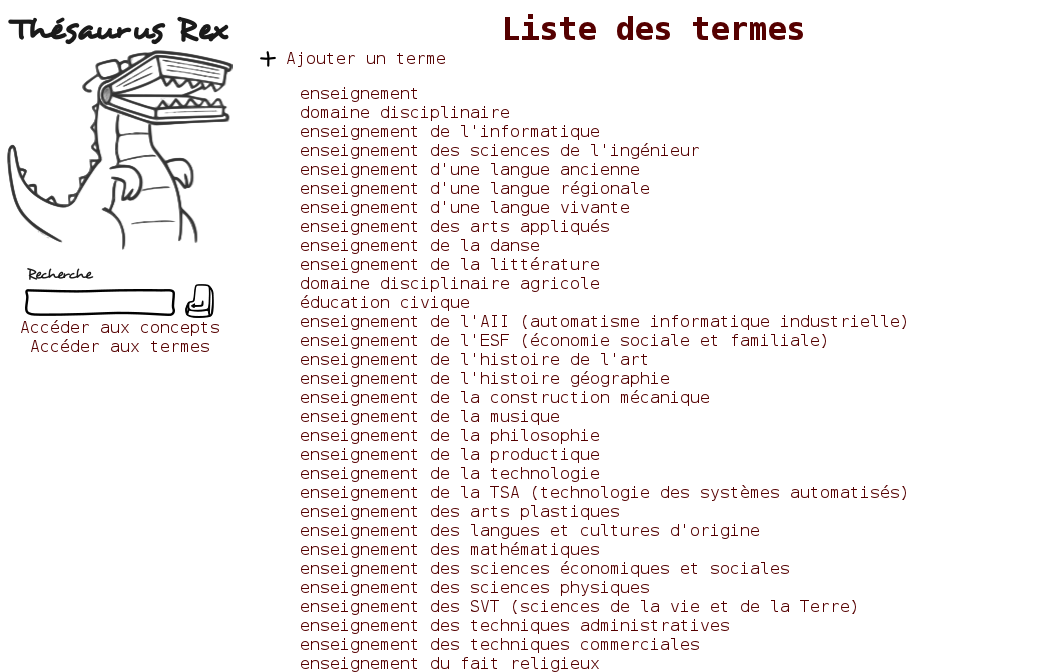
\includegraphics[width=\textwidth]{files/screen_termes}
\end{center}
\caption{Aperçu de la page de liste des termes.}
\end{figure}

\subsubsection{Modification d'un terme}
\begin{figure}[H]
\begin{center}
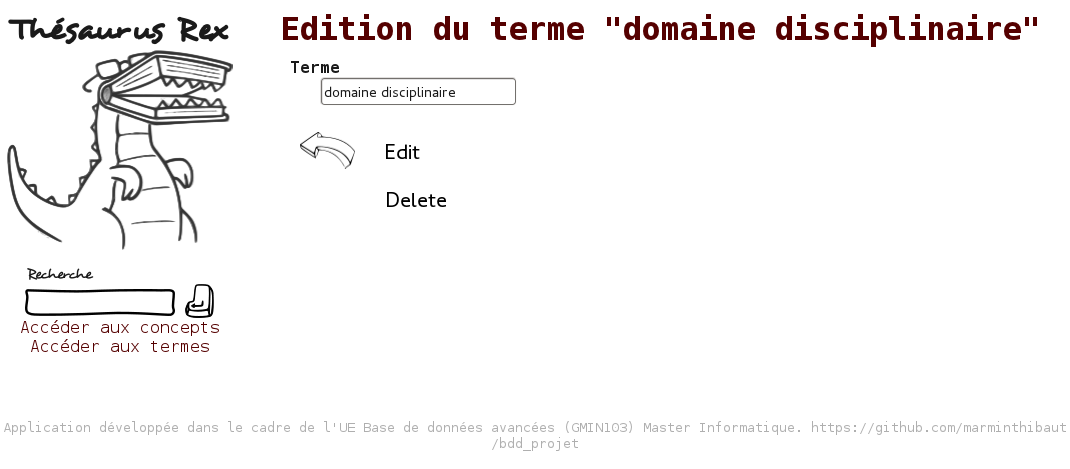
\includegraphics[width=\textwidth]{files/screen_terme_edit}
\end{center}
\caption{Formulaire d'édition d'un terme.}
\end{figure}
